\documentclass[cn, math=cm]{elegantbook}	
% [simple]下文档类的环境很简洁,不建议使用
% 要使用中文必须指定文档的Lang。即使用[lang=cn]或[cn]
% 使用[section]可以更改公式编号的格式,如0.0.1。默认是0.1
% math=[]。可以指定数学环境的字体。缺省cm
\usepackage{hyperref}
% 插入超链接
\usetikzlibrary{animations}

\setcounter{tocdepth}{2}
\cover{Picture/海琴烟.jpg}
\title{Learn Elegant\LaTeX}
\date{\today}
\author{Eureka}


\begin{document}
	\maketitle
	\tableofcontents
	\newpage
	\clearpage

	\section{环境的测试}
	\subsection{测试中文和Theorem 环境}
	% Elegant下的数学环境还是需要数学环境的命令。如$$, $$$$, align等 
     \begin{theorem}[Fourier serise]\label{label-1}
     % label的格式不能用:\begin{theorem}{Fourier serise}
     % 这样使用\ref{thm:label-1}仍然不能够引用。
		we have the Fourier fomular that :
		\begin{align}
		f\sim\frac{a_0}{2}\sum_{i=1}^{\infty}{[a_n\cos(nx)+b_n\sin(nx)]}
		\end{align}
		\end{theorem}
		\subsection{引理环境}
		\begin{lemma}
			This is a lamma test
		\end{lemma}
		\subsection{推论环境}
		\begin{corollary}
			This is a corollary
		\end{corollary}
		\subsection{命题环境}
		\begin{proposition}
			This is a proposition
		\end{proposition}
		\subsection{章节摘要环境}
		\begin{introduction}
		\item 1 .Definition of Theorem
		\item 2 .Ask for help\\
		% \\代表换行(产生空行),默认顺序:从上倒下,从左到右
		\item 3 .Optimization Problem
		\item 4 .Property of Cauchy Series
		\item 5 .Angle of Corner
	\end{introduction}
	\subsection{标签的引用}
	所以从上边我们可以看出定理\ref{label-1}指出了函数的展开形式。
	\ref{label-1}
	\newpage
	\subsection{definition环境的测试}

	\begin{definition}
	     设$f(x)$是定义在$[a,b]$上的有界函数,在$[a, b]$上任取分点$\{x_i\}^n_{i=0}$,做一种划分:\\
        $$P:a=x_0<x_1<x_2<\cdots<x_{n-1}<x_n=b$$
        并且任取点$\xi_i\in[x_{i-1},x_i]$.记小区间的长度为$\Delta x_{i-1}=x_i-x_{i-1}$,并令$\lambda=\max\limits_{1\le i\le n}(\Delta x_i)$,若当$\lambda\to 0$时,极限
        \begin{equation}
            \lim\limits_{\lambda\to 0}{\sum_{i}^{n}{f(\xi_i)\Delta x_i}}\nonumber
        \end{equation}
        存在,并且与划分P无关,又对$\xi_i$的取法无关,则称$f(x)$在$[a, b]$上Riemann可积,和式
        \begin{equation}
        S_n= \sum_{i=1}^{n}{f(\xi_i\Delta x_i)}\nonumber
        \end{equation}

        称为Riemann和,其极限$I$称为$f(x)$在$[a, b]$上的定积分,记为:
        \begin{equation}
        I=\int_{a}^{b}{f(x) dx}\nonumber
        \end{equation}
	\end{definition}

	\section{插入代码}
	% 在lstlisting中的内容会保持原样输出
	\begin{lstlisting}[language=Python]
		import matplotlib.pyplot as plt
		import numpy as np
		import time

		plt.rcParams['font.sans-serif'] = ['SimHei']
		plt.rcParams['axes.unicode_minus'] = False
		# 注:不能使用中文,latex会报错
		# 也可以不适用这句话直接使用$公式$,这样就能够表示中文
		plt.rc('text', usetex=True)


		# plt.rcParams.update({
		#     "pgf.texsystem": "xelatex",
		#     "text.usetex": True,    # use default xelatex
		# })

		# 打开交互模式
		# 需要关闭pycharm自带的 show plots in tool window
		plt.ion()
		# 读取当前的时间
		t0 = time.time()

		# 使用类似动画的方法,把动画一帧一帧的显示出来
		while True:
		    plt.clf()   # 清除上一帧

		    # 第一个子图
		    plt.subplot(1, 2, 1)    # 一行两列
		    plt.title("cuevr figure")
		    plt.xlabel("time(s)")
		    plt.ylabel("value")
		    # 坐标轴范围
		    plt.ylim(-2, 2)
		    t = time.time() - t0
		    x = np.arange(t, t+8, 0.01)
		    y1 = np.sin(x)
		    y2 = np.sin(x*3)/3
		    y3 = np.sin(x*5)/5
		    y4 = np.sin(x*7)/7

		    # 绘制每一帧
		    plt.plot(x, y1, color="r", linestyle=":", label=r"$y=\frac{\sin(x)}{1}$")
		    plt.plot(x, y2, color="g", linestyle=":", label=r"$y=\frac{\sin(2x)}{2}$")
		    plt.plot(x, y3, color="b", linestyle=":", label=r"$y=\frac{\sin(3x)}{3}$")
		    plt.plot(x, y4, color="#0ff", linestyle=":", label=r"$y=\frac{\sin(4x)}{4}$")
		    # 添加图注
		    plt.legend(loc="upper right")

		    # 第二个子图
		    plt.subplot(1, 2, 2)
		    y5 = y1 + y2 + y3 + y4
		    plt.plot(x, y5, color="b", linestyle="-", label="Accumalate")
		    # 添加图注
		    plt.legend(loc="upper right")

		    plt.pause(0.01)
	\end{lstlisting}

	\section{TIKZ基础}
	\subsection{绘制图像}
	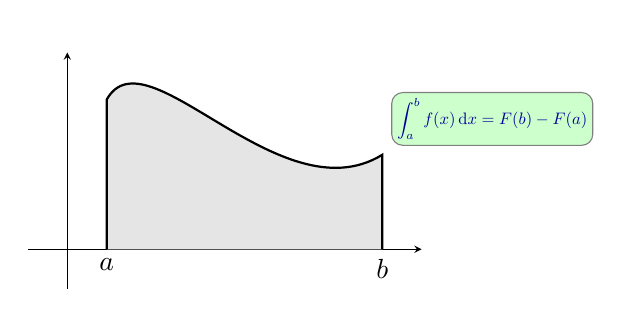
\begin{tikzpicture}
		\draw[-stealth,line width=0.2pt] (-0.5,0) -- (4.5,0);
		\draw[-stealth,line width=0.2pt] (0,-0.5) -- (0,2.5);
		\coordinate (a)
		at (0.5,1.9);
		\coordinate (b)
		at (4,1.2);
		\node[below] (a0) at (a |- 0,0) {$a$};
		\node[below] (b0) at (b |- 0,0) {$b$};
		\filldraw[fill=gray!20,draw,thick]
		(a0) -- (a) .. controls (1,2.8) and (2.7,0.4) .. (b) -- (b0) -- cycle;
		\node[above right,outer sep=0.2cm, rounded corners,
		fill=green!20,draw=gray,text=blue!60!black,scale=0.6]
		at (b) {$\displaystyle \int_a^b {f(x)\,\mathrm{d}x} = F(b) - F(a)$};
	\end{tikzpicture}
	\subsection{绘制动画}
		
	\section{参考文献}
	测试参考文献引用

	本篇文章引用的文献为\cite{kearon1998noninvasive}
	% 引用文献不能用如下的方式了
	% \bibliography{reference}
	% \bibliography{reference}
	% 正确的打印引用文献的方法
	\printbibliography[heading=bibintoc, title=参考文献]

	\section{插入超链接}
	\section*{参考资料}
	\begin{itemize}
	  \item \href{https://packagecontrol.io/installation}{Package Control Installation}.
	  \item \href{https://latextools.readthedocs.io/en/latest/install/}{LaTeXTools Installation}
	  \item \href{https://liam.page/2013/11/11/Sublime-elegant/}{极致优雅——Sublime Text 简介/入门/技巧}
	  \item \href{https://ddswhu.me/posts/2018-06/sublime-text-for-latex/}{Configure Sublime Text 3 as LaTeX IDE}
	  \item \href{http://www.latexstudio.net/archives/51449.html}{LaTeX 技巧 935: Sublime Text 下的 LaTeX 及高级应用}
	\end{itemize}
\end{document}